\chapter{РЕШЕНИЕ ПРИКЛАДНОЙ ЗАДАЧИ}

\section{Постановка прикладной задачи}

Разработать систему хранения  документов с составлением реферата документа и выделением ключевых слов для упрощения индексации и поиска документов. 

\section{Решение прикладной задачи}

На основе разработанного программного обеспечения описанная выше прикладная задача имеет следующее решение. Научному сотруднику предлагается графический интерфейс для загрузки документов в базу данных и графический интерфейс для ознакомления со всей базой данных документов. На основе уже разработанного программного обеспечения для поиска в базе данных. Одним из таких программных продуктов является бесплатный клиент базы данных $mongoDB$ с открытым исходным кодом \textit{MongoDB Compass}\hyperref[itm:compass]{[\ref{itm:compass}]}.

Приложение, разработанное в этой главе вместе с инструментом для фильтрации результатов в базе данных позволяют организовать хранилище документов, которое позволит быстро найти нужные документы.

Графический интерфейс разработанного программного обеспечения представлен на рисунках \hyperref[fig:front_main]{\ref{fig:front_main}} и \hyperref[fig:front_all]{\ref{fig:front_all}}

\begin{figure}[H]
\centering
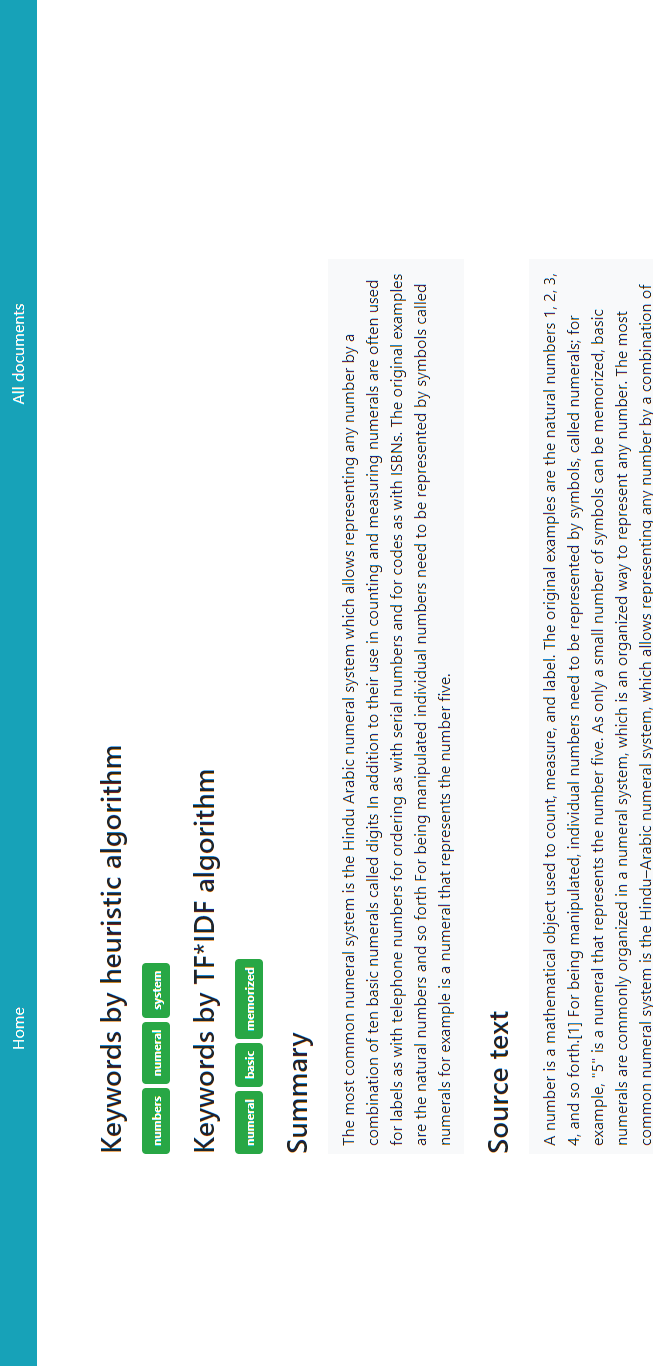
\includegraphics[height=0.85\textheight]{alldocs.png}
\caption{Графический интерфейс страницы для отображения всех документов}
\label{fig:front_all}
\end{figure}

\begin{figure}[H]
\centering
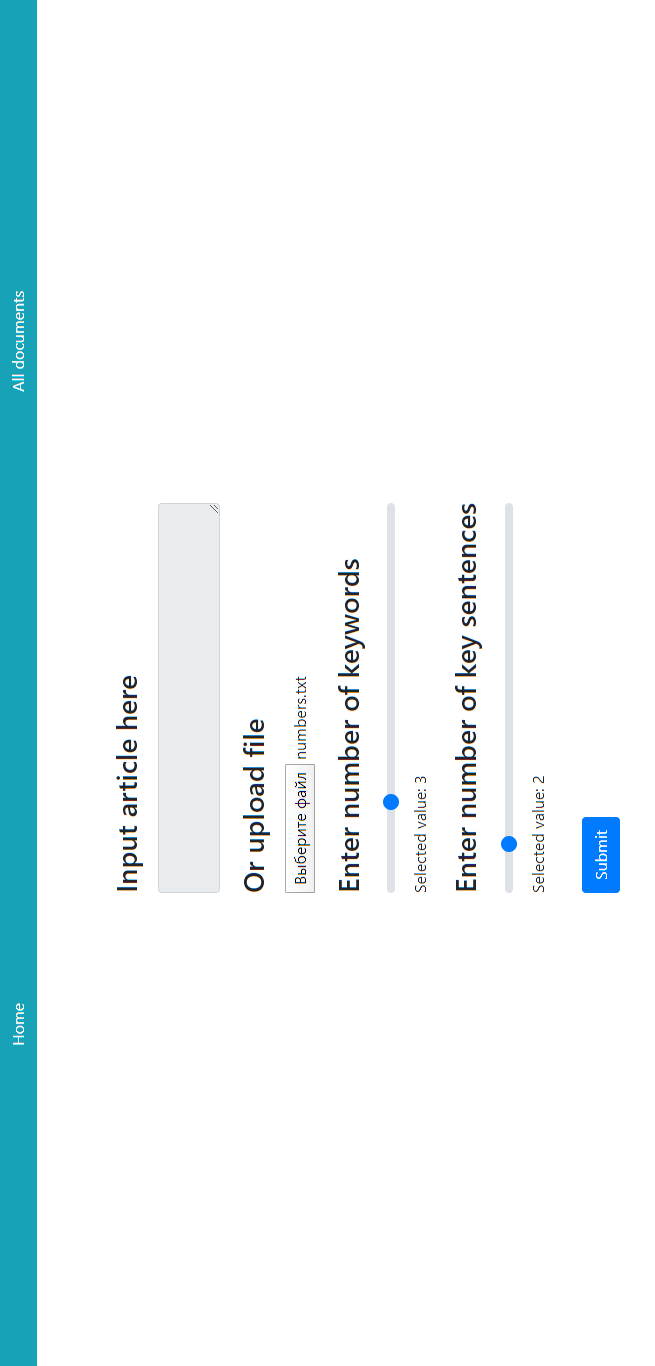
\includegraphics[height=0.8\textheight]{mainpage.png}
\caption{Графический интерфейс главной страницы}
\label{fig:front_main}
\end{figure}

Результаты работы программы для текста, представленного в приложении \hyperref[app:capitalism]{\ref{app:capitalism}}, можно увидеть на рисунке \hyperref[fig:res_capitalism]{\ref{fig:res_capitalism}}.

\begin{figure}[H]
\centering
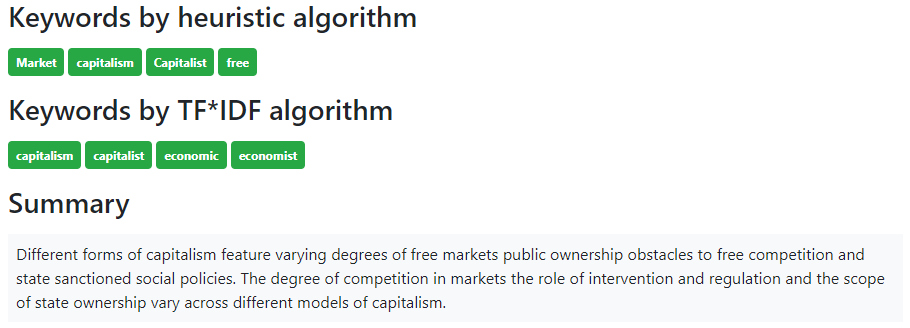
\includegraphics[width=\textwidth]{capitalism.png}
\caption{Результат работы программы для текста из приложения \hyperref[app:capitalism]{\ref{app:capitalism}}}
\label{fig:res_capitalism}
\end{figure}

Пример использования программы \textit{MongoDB Compass} для поиска документов в базе данных по ключевым словам представлен на рисунке \hyperref[fig:mongo_capitalism]{\ref{fig:mongo_capitalism}}.

\begin{figure}[H]
\centering
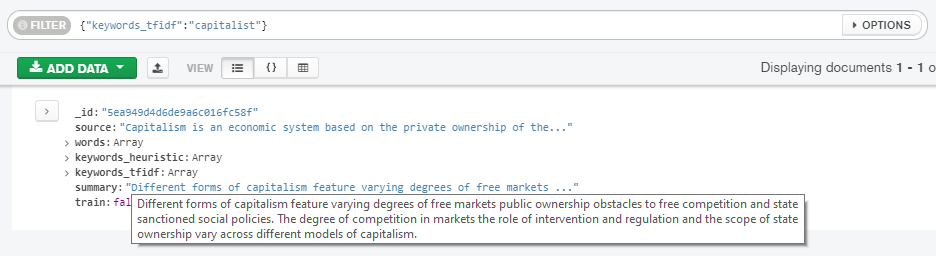
\includegraphics[width=\textwidth]{mongofilter.png}
\caption{Использование \textit{MongoDB Compass} для поиска документов по ключевым словам}
\label{fig:mongo_capitalism}
\end{figure}

\section{Анализ результатов}

Пользователями системы будут являться, например, научные работники, которым необходимо обращаться к собственной, закрытой базе данных документов. Ключевые слова помогут найти статью по нужной теме, а резюме документа поможет понять смысл текста. Вообще говоря, разработанное программное обеспечение может использоваться в любых сферах, где требуется хранение и поиск документов в собственной базе данных. Система является самообучаемой и при добавлении новых документов в базу данных, она корректирует коэффициенты, используемые для подсчета важности слов в тексте.

Однако система не подойдет для хранения статей или книг большого объема, так как невозможно подытожить целую книгу, выделив из нее несколько предложений. Плюсом данной системы является горизонтальная масштабируемость, которая позволяет увеличивать производительность системы с помощью добавления новых вычислительных устройств, а не улучшения старых ЭВМ.

В текущей версии программы выделение ключевых используются два алгоритма, так как эвристический алгоритм показывает лучшие результаты на текстах малого объема, а алгоритм на основе машинного обучения лучше находит ключевые слова в текстах среднего объема. В итоговом продукте можно выбирать алгоритм на основе размера входного текста, однако в текущей версии программы каждому тексту в демонстративных целях присваивается два набора ключевых слов.

\section{Выводы}

В четвертой главе были получены следующие результаты:
\begin{itemize}
\item сформулированы прикладная задача анализа неструктурированного текста;
\item представлено ее решение на основе разработанного программного инструментария;
\item представлен анализ результатов и пути использования разработанных программ в различных прикладных областях. 
\end{itemize}
